\subsection{$\tau$ validation on binary Mnist digit classification}

\subsubsection{Motivation}

The parameter \(\tau\) in the LIF neuron model influences the neuron's temporal dynamics, governing both its spike response width and the timing of its peak response, as discussed in section \ref{}. 
Let's delve deeper into the impact of varying \(\tau\) values on our current classification task.


\subsubsection{Experimental Framework}

The main aim of this experiment is to assess how the convolution-based Tempotron model performs on Mnist odd and even digits, particularly when adjusting the values of $\tau$.

\subsubsection{Input Data}

The Mnist Digits dataset was utilized, separating it based on odd and even digits, represented by a binary label. Each $28 \times 28$ image was transformed into a 784-length vector, normalized to lie within the range [0, 1]. The data was then encoded using the rate encoding method detailed in section \ref{ssec:rate-encoding-method}.


\subsubsection{Model Architecture}

The Convolution-based Tempotron model's design and operational mechanics are detailed in section \ref{sssec:training-conv-cost} on \textbf{Methods}.


\subsubsection{Procedure}

For each selected $\tau$ value, multiple experimental trials were executed, each undergoing a preset number of learning iterations (or until training convergence), processing data in specified batch sizes.

\subsubsection{Parameter Descriptions}

\begin{enumerate}
    \item \textbf{Duration \( T \): 500 ms} \\
    Represents the length of time for which the model will simulate the neural dynamics for each given input pattern.
    
    \item \textbf{Time step \( dt \): 1 ms} \\
    The sampling time at which we "measure" the experiment.
    
    \item \textbf{Potential Scaling Factor \( V_0 \): 2.12} 
    
    \item \textbf{Firing threshold \( V_{th} \): 1} \\
    The potential level at which a neuron emits a spike. When the neuron's membrane potential exceeds $V_{th}$, it "fires" or produces an output spike.
    
    \item \textbf{Exponent scaling factor \( \beta \): 50} \\
    The coefficient of the exponent in the output layer.

    \item \textbf{Max rate \( R \): 20 Hz} \\
    Determines the maximum rate at which a neuron fires.
    
    \item \textbf{Output layer size: 1 neuron} \\
    Indicates the number of neurons in the model's final layer, which produces the final decision or classification.
    
    \item \textbf{Maximum iterations: 750} 

    \item \textbf{Batch size: 64} \\
    Dictates how many input patterns are processed simultaneously before updating the model's internal parameters. 

\end{enumerate}

\subsubsection{Results}

\begin{figure}[H]
    \centering
    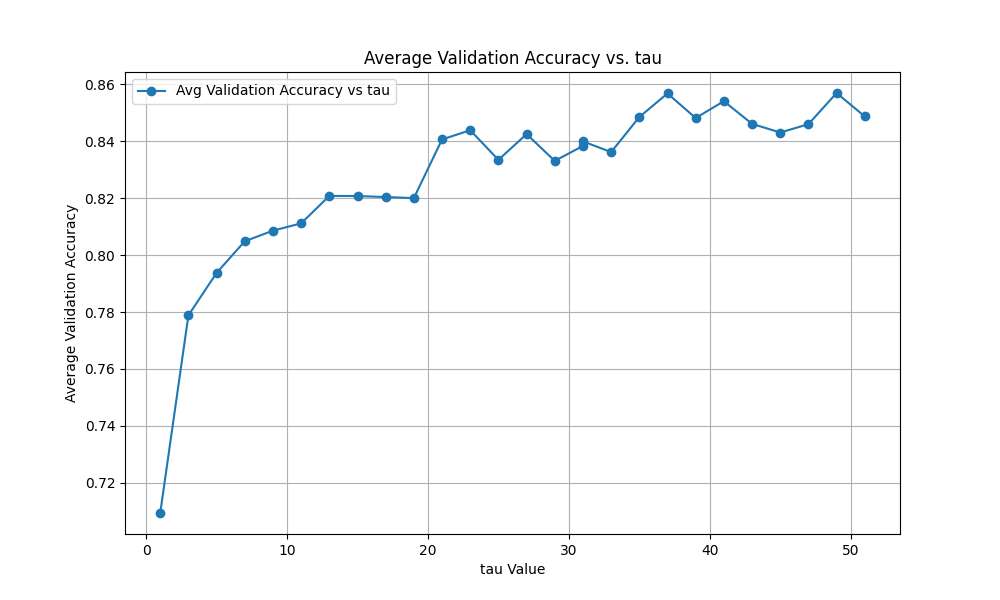
\includegraphics[width=0.8\linewidth]{results/graphs/tau-validation.png}
    \caption{Average test accuracy as a function of $\tau$}
    \label{fig:tau-validation}
\end{figure}


\subsubsection{Observation}

